% =====================================================================
\section{Resultados}
\label{sec:resultados}

Esta sección presenta los cuadrantes que recomienda el modelo para los tres meses de referencia. La Sección~\ref{sec:analisis} analiza cómo cambian al variar los supuestos.

\begin{table}[ht]
\centering\small
\caption{Resultados de los tres meses de referencia (datos sintéticos). Todos los indicadores se calculan a partir del cuadrante $x$. Rango de carga de festivos: $e^{\protect\max} - e^{\protect\min}$ antes y después del mes.}
\label{tab:base}
\setlength{\tabcolsep}{5pt}
\begin{tabular}{@{}lcccccc@{}}
\toprule
 & \multicolumn{2}{c}{Enero 2027} & \multicolumn{2}{c}{Diciembre 2026} & \multicolumn{2}{c}{Agosto 2027} \\
\cmidrule(lr){2-3}\cmidrule(lr){4-5}\cmidrule(lr){6-7}
Escenario & A & B & A & B & A & B \\
\midrule
Plazas de guardia sin cubrir ($h$)            & \textbf{0} & 37 & 5 & 37 & 24 & 47 \\
Mayores que faltan ($h^S$)                    & 0 & 0 & 0 & 2 & 0 & 4 \\
Residentes que faltan en planta ($h^P$)       & 0 & 0 & 1 & 0 & 15 & 19 \\
Guardias por debajo del mínimo ($h^G$)        & 0 & 0 & 0 & 0 & 0 & 0 \\
\textbf{Requisitos incumplidos $f_1$}         & \textbf{0} & \textbf{37} & \textbf{6} & \textbf{39} & \textbf{39} & \textbf{70} \\
Peticiones incumplidas / total                & 0/17 & 0/17 & 0/12 & 0/12 & 0/21 & 0/21 \\
Rango de carga de festivos antes del mes      & 21,7 & 21,7 & 27,5 & 27,5 & 10,3 & 10,3 \\
Rango de carga de festivos después ($f_3$)    & 14,8 & 17,1 & 23,1 & 23,1 & 9,8 & 9,8 \\
Patrones «día sí, día no» ($f_4$)             & 1 & 0 & 0 & 0 & 0 & 0 \\
Guardias por residente (mín.--máx.)           & 5--7 & 4--4 & 4--7 & 4--4 & 2--7 & 2--4 \\
Mín. de residentes en planta (día laborable)  & 9 & 9 & 8 & 9 & 6 & 6 \\
Tiempo de resolución (s)                      & 0,3 & 0,4 & 0,3 & 0,3 & 0,3 & 0,3 \\
\bottomrule
\end{tabular}
\end{table}

\subsection{Mes base: enero de 2027}

En el régimen actual (escenario A) el modelo encuentra un cuadrante que \textbf{cumple todos los requisitos} (Tabla~\ref{tab:base} y Figura~\ref{fig:roster}): cubre las 93 plazas con al menos un residente mayor en cada guardia de urgencias, nunca deja menos de 9 residentes en planta, respeta las 17 peticiones de días libres y solo deja un patrón «guardia, libre, guardia». Cada residente hace entre 5 y 7 guardias. El modelo tiene 1\,352 variables (758 binarias) y 1\,393 restricciones y se resuelve en menos de medio segundo, frente a las horas que lleva hacerlo a mano.

\begin{figure}[ht]
\centering
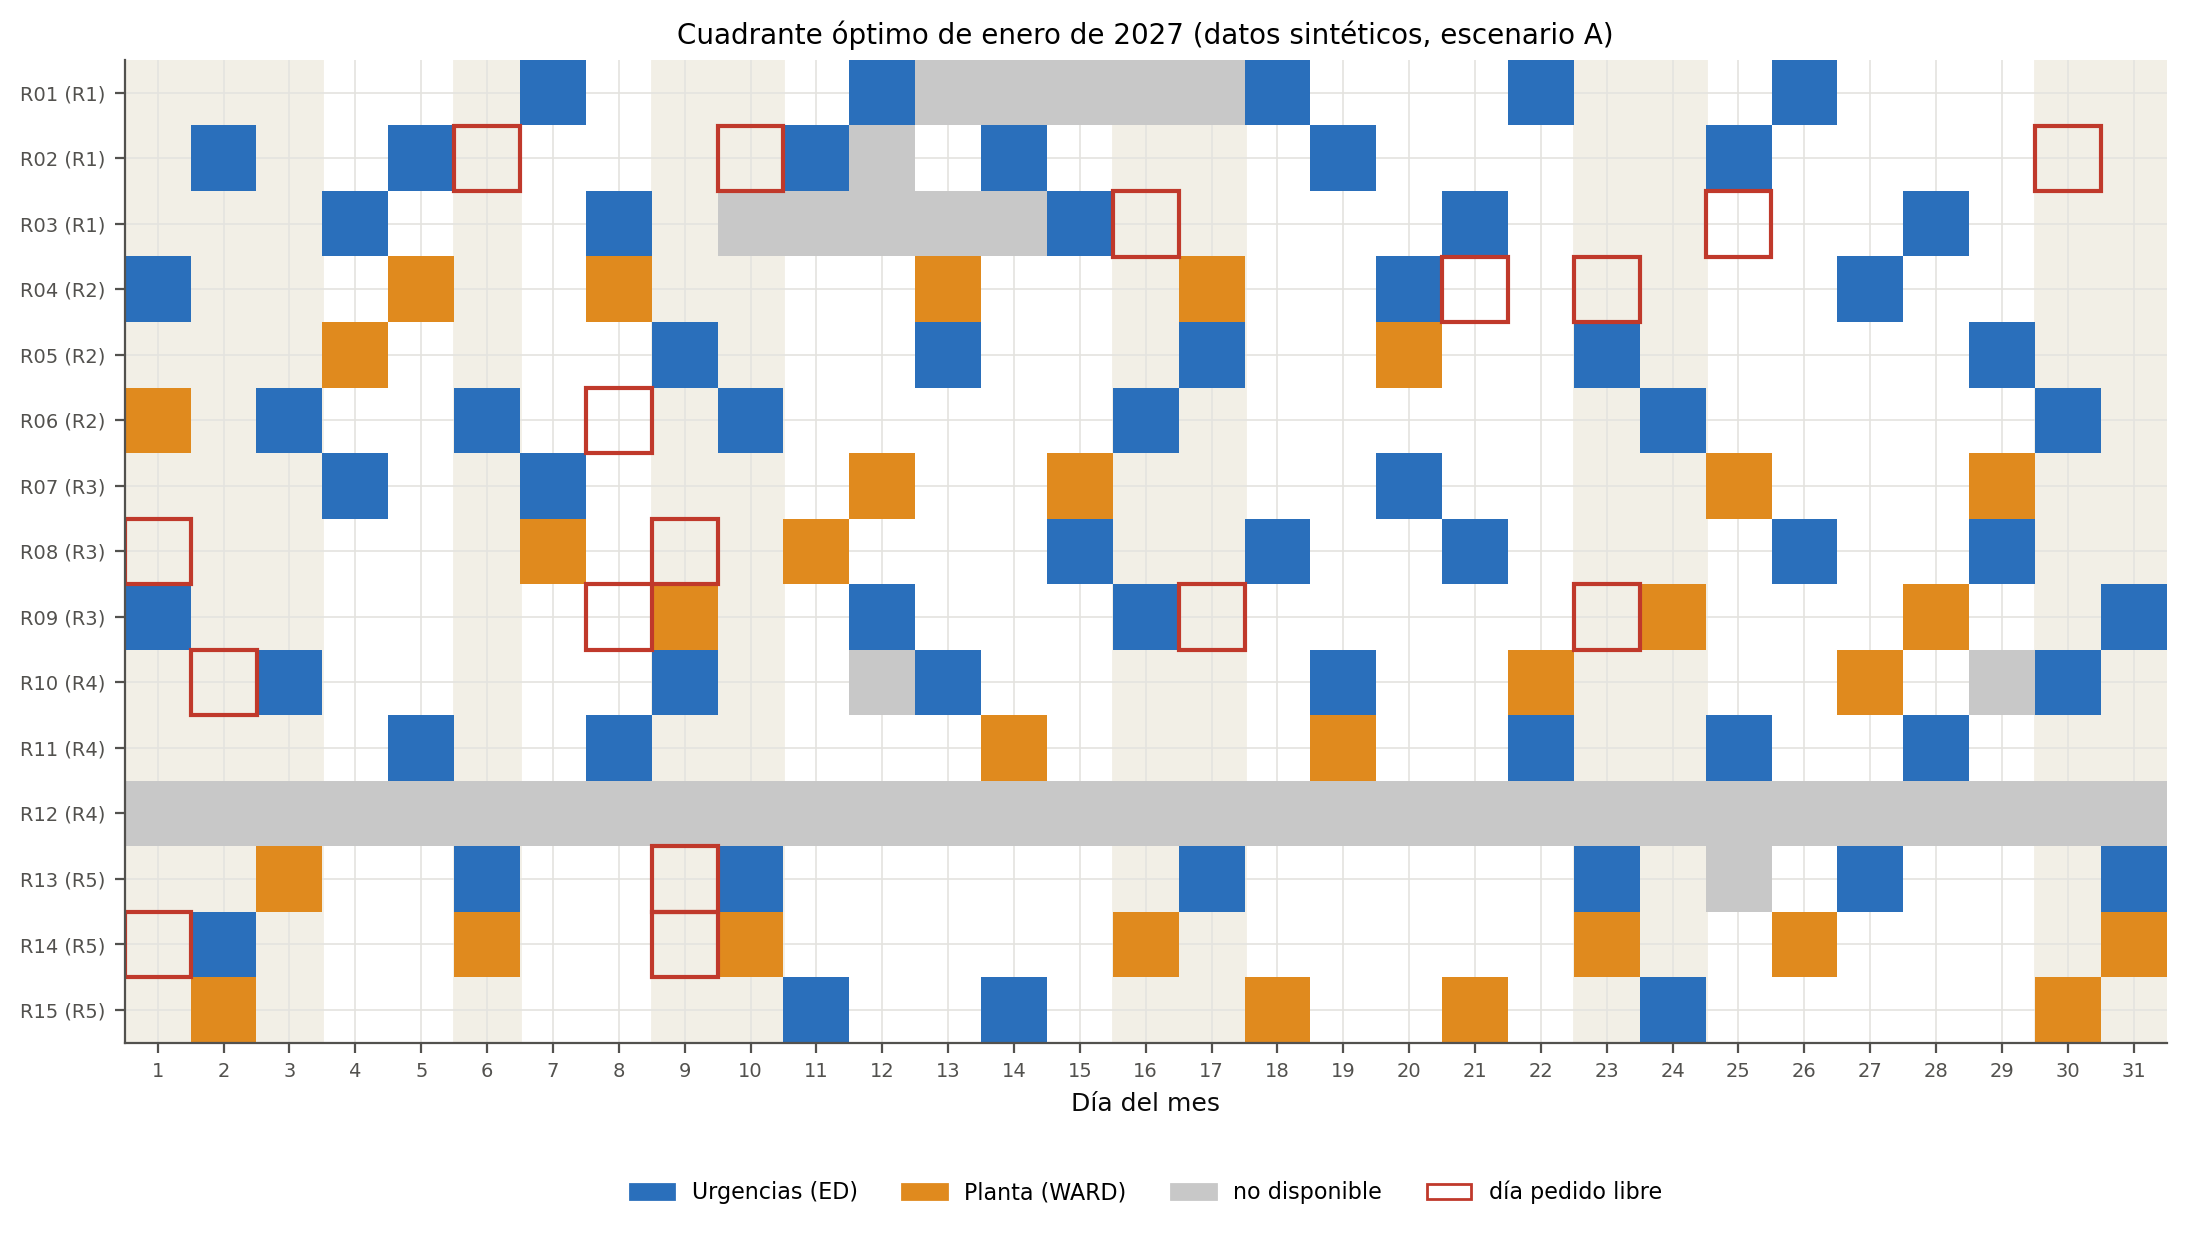
\includegraphics[width=\linewidth]{final_roster_jan2027.png}
\caption{Cuadrante óptimo de enero de 2027 (escenario A). Cada fila es un residente (entre paréntesis, su año de residencia) y cada columna un día. Azul: guardia de urgencias; naranja: guardia de planta; gris: no disponible (vacaciones, rotación externa o curso); recuadro rojo: día pedido libre; columnas sombreadas: fines de semana y festivos.}
\label{fig:roster}
\end{figure}

\paragraph{Equidad.} El modelo asigna los fines de semana y festivos de enero a quienes llevaban menos carga acumulada (Figura~\ref{fig:fairness}): la diferencia entre el residente más cargado y el menos cargado baja de 21,7 a 14,8 guardias normalizadas. No baja más porque el residente más cargado (R07) ya acumula 32 guardias normalizadas: aunque no haga ningún festivo en enero, a los menos cargados no les da tiempo a alcanzarle en un solo mes. Esto es lo que motiva el análisis de varios meses seguidos de la Sección~\ref{sec:equidad}.

\begin{figure}[ht]
\centering
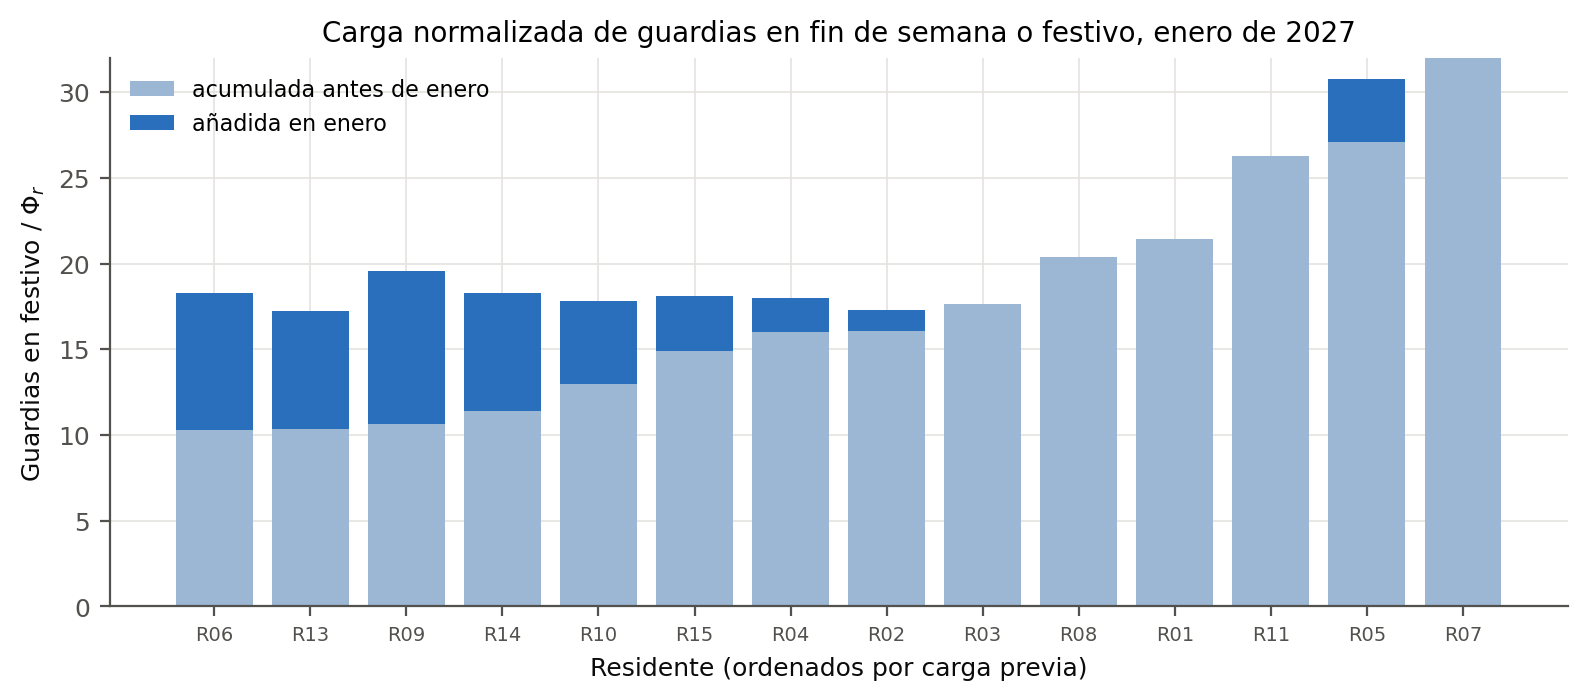
\includegraphics[width=0.78\linewidth]{final_fairness_jan2027.png}
\caption{Carga normalizada de guardias en fin de semana o festivo, $(H_r + \sum_{d \in \mathcal{F}} y_{rd}) / \Phi_r$: acumulada antes de enero (azul claro) y añadida en enero (azul oscuro). Los residentes están ordenados por su carga previa.}
\label{fig:fairness}
\end{figure}

\subsection{Meses difíciles y régimen de 2027}

\paragraph{Diciembre.} Aunque la capacidad nominal es la misma que en enero (98 guardias para 93 plazas), quedan 5 plazas sin cubrir y falta un residente en planta un día. Las vacaciones de Navidad se concentran en las mismas semanas y, con la regla de descanso, quienes quedan no pueden hacer guardias suficientes en esos días: la capacidad real es menor que la nominal.

\paragraph{Agosto.} Con ocho residentes de vacaciones dos semanas, quedan 24 plazas sin cubrir y faltan 15 residentes-día en planta; 7 de esos 15 faltarían aunque nadie hiciera guardias (déficit estructural). Los huecos se concentran en las tres primeras semanas, cuando hay entre 6 y 11 residentes disponibles (frente a 13 o 14 al final del mes), y caen siempre en guardias de domingo a jueves, nunca en viernes ni sábado. La razón es la restricción (9): quien hace guardia un viernes o un sábado sale de guardia en fin de semana y no resta personal de planta, mientras que una guardia de domingo a jueves deja un saliente al día siguiente en una planta que ya va corta. El modelo deja sin cubrir justo las guardias que más cuestan a la actividad ordinaria. La Sección~\ref{sec:planta} analiza este intercambio.

\paragraph{Escenario B (RD 951/2026).} Con un máximo de cuatro guardias de 17~h por residente, los 14 residentes disponibles solo pueden cubrir $14 \times 4 = 56$ de las 93 plazas: quedan 37 sin cubrir en enero y diciembre, y en agosto el déficit total llega a 70 personas. Con la plantilla actual el régimen de 2027 no es viable.

% =====================================================================
\section{Análisis de los resultados}
\label{sec:analisis}

Un único cuadrante óptimo responde a la pregunta P1. Para las preguntas de planificación (P2 a P4) resolvemos el modelo más de 500 veces cambiando la plantilla, el límite mensual, el requisito de planta, la prioridad de los objetivos y la forma de medir la equidad. Cada experimento cambia un único elemento respecto al caso base; todos los cuadrantes se validan de forma independiente.

\subsection{¿Cuántos residentes necesita el servicio?}
\label{sec:plantilla}

Para cada mes y régimen normativo quitamos de 1 a 4 residentes (cinco sorteos aleatorios para cada número) o añadimos de 1 a 12 residentes sintéticos totalmente disponibles. Además del régimen actual (A, 7 guardias) y del RD 951/2026 (B), estudiamos dos acuerdos locales más estrictos que el máximo legal (6 y 5 guardias al mes). La Figura~\ref{fig:plantilla} muestra los requisitos incumplidos $f_1$ y la Tabla~\ref{tab:plantilla} la plantilla mínima.

\begin{figure}[ht]
\centering
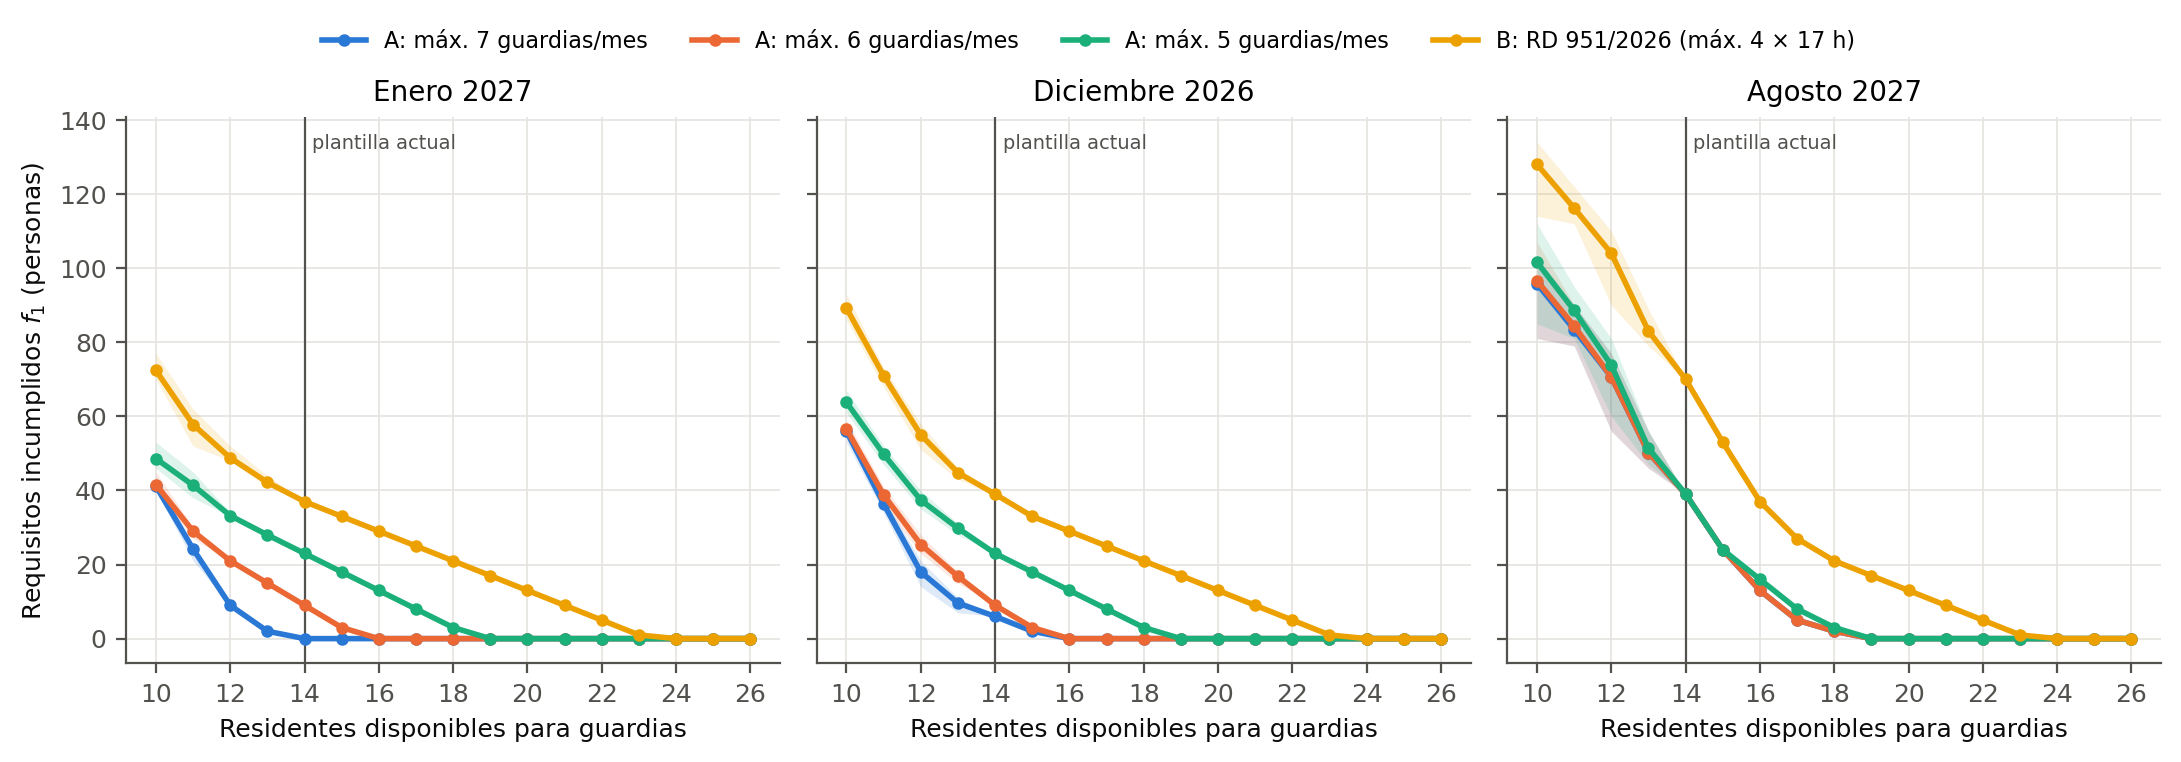
\includegraphics[width=\linewidth]{final_staffing_vs_regime.png}
\caption{Requisitos incumplidos $f_1$ (plazas de guardia, mayores y residentes en planta que faltan) según el número de residentes disponibles para guardias y el límite mensual. A la izquierda de la línea vertical se quitan residentes (media de cinco sorteos; la banda indica el mínimo y el máximo); a la derecha se añaden residentes totalmente disponibles.}
\label{fig:plantilla}
\end{figure}

\begin{table}[ht]
\centering\small
\caption{Residentes disponibles para guardias necesarios para cumplir todos los requisitos ($f_1 = 0$) y, entre paréntesis, para cubrir todas las guardias si se permite reducir la actividad ordinaria. Cota aritmética: $\lceil 93 / \text{máximo mensual} \rceil$. Hoy hay 14.}
\label{tab:plantilla}
\begin{tabular}{@{}lcccc@{}}
\toprule
Régimen & Cota aritmética & Enero 2027 & Diciembre 2026 & Agosto 2027 \\
\midrule
A: máximo 7 guardias (actual)  & 14 & \textbf{14} (14) & \textbf{16} (14) & \textbf{19} (14) \\
A: máximo 6 guardias           & 16 & 16 (16) & 16 (16) & 19 (16) \\
A: máximo 5 guardias           & 19 & 19 (19) & 19 (19) & 19 (19) \\
B: RD 951/2026 (4 de 17 h)     & 24 & \textbf{24} (24) & \textbf{24} (24) & \textbf{24} (24) \\
\bottomrule
\end{tabular}
\end{table}

\paragraph{Lo que recomienda el modelo.}
\begin{itemize}
  \item \textbf{Hoy el servicio no tiene margen.} En enero bastan los 14 residentes disponibles, pero con uno menos ya quedan 2 plazas sin cubrir y todos tienen que hacer el máximo de 7 guardias. El déficit crece cada vez más deprisa: 9 requisitos con dos residentes menos y 41 con cuatro menos, porque a partir de tres ausencias empieza a faltar también personal en planta.
  \item \textbf{El RD 951/2026 exige unos 10 residentes más} (de 14 a 24, un 71\,\% más) para mantener la estructura de guardias actual. En B el cuello de botella es puramente aritmético: cada residente aporta como mucho 4 guardias, cada residente añadido reduce el déficit exactamente en 4 plazas y el modelo alcanza la cota $\lceil 93/4 \rceil = 24$ en los tres meses. La alternativa a contratar es rediseñar las guardias (menos plazas de residente, más adjuntos), y el modelo permite evaluar cada propuesta en segundos.
  \item \textbf{En los meses difíciles el problema no es aritmético.} En diciembre y agosto la cota aritmética del régimen actual (14) no basta: hacen falta 16 y 19 residentes para cumplirlo todo, porque las vacaciones coinciden en los mismos días y cada guardia deja un saliente. Este es el tipo de respuesta que no se obtiene con una hoja de cálculo. Sin embargo, si el servicio acepta reducir la actividad ordinaria, en ambos meses \emph{se pueden cubrir todas las guardias con la plantilla actual} (cifras entre paréntesis): la decisión es de gestión y se analiza en la Sección~\ref{sec:planta}.
  \item \textbf{Un acuerdo local de 5 guardias} costaría tanto como agosto en cualquier mes (19 residentes): las restricciones de calendario dejan de importar porque domina el límite mensual.
\end{itemize}

\subsection{¿Importa quién falta?}

Quitamos dos residentes del mismo año de residencia, probando todas las parejas posibles. En enero el resultado no depende del año: cualquier pareja deja exactamente 9 plazas sin cubrir, que es la diferencia entre las 93 plazas y las $12 \times 7 = 84$ guardias que pueden hacer los 12 restantes. En agosto el déficit varía entre 56 y 77, pero tampoco lo explica el año de residencia, sino la disponibilidad: perder a dos residentes que ya tenían vacaciones cuesta 56--58 requisitos; perder a uno que estaba disponible todo el mes, 66--67, y perder a dos, 77. Con 9 mayores de 15 la exigencia de un mayor por guardia nunca es el problema. \textbf{El recurso escaso son los días-residente disponibles}, así que repartir las vacaciones a lo largo del verano importa más que quién las coge.

\subsection{Guardias frente a actividad ordinaria: el coste de los salientes}
\label{sec:planta}

El objetivo $f_1$ suma con el mismo peso una plaza de guardia sin cubrir y un residente que falta en planta. Por la restricción (9), cada guardia de domingo a jueves deja un saliente que no trabaja al día siguiente. Cuando la planta va justa, cubrir una guardia más cuesta exactamente un residente menos en planta, y el modelo es indiferente entre ambas opciones. Lo comprobamos con una variante que cubre primero las guardias y después la planta (dos niveles lexicográficos en lugar de uno).

\begin{figure}[ht]
\centering
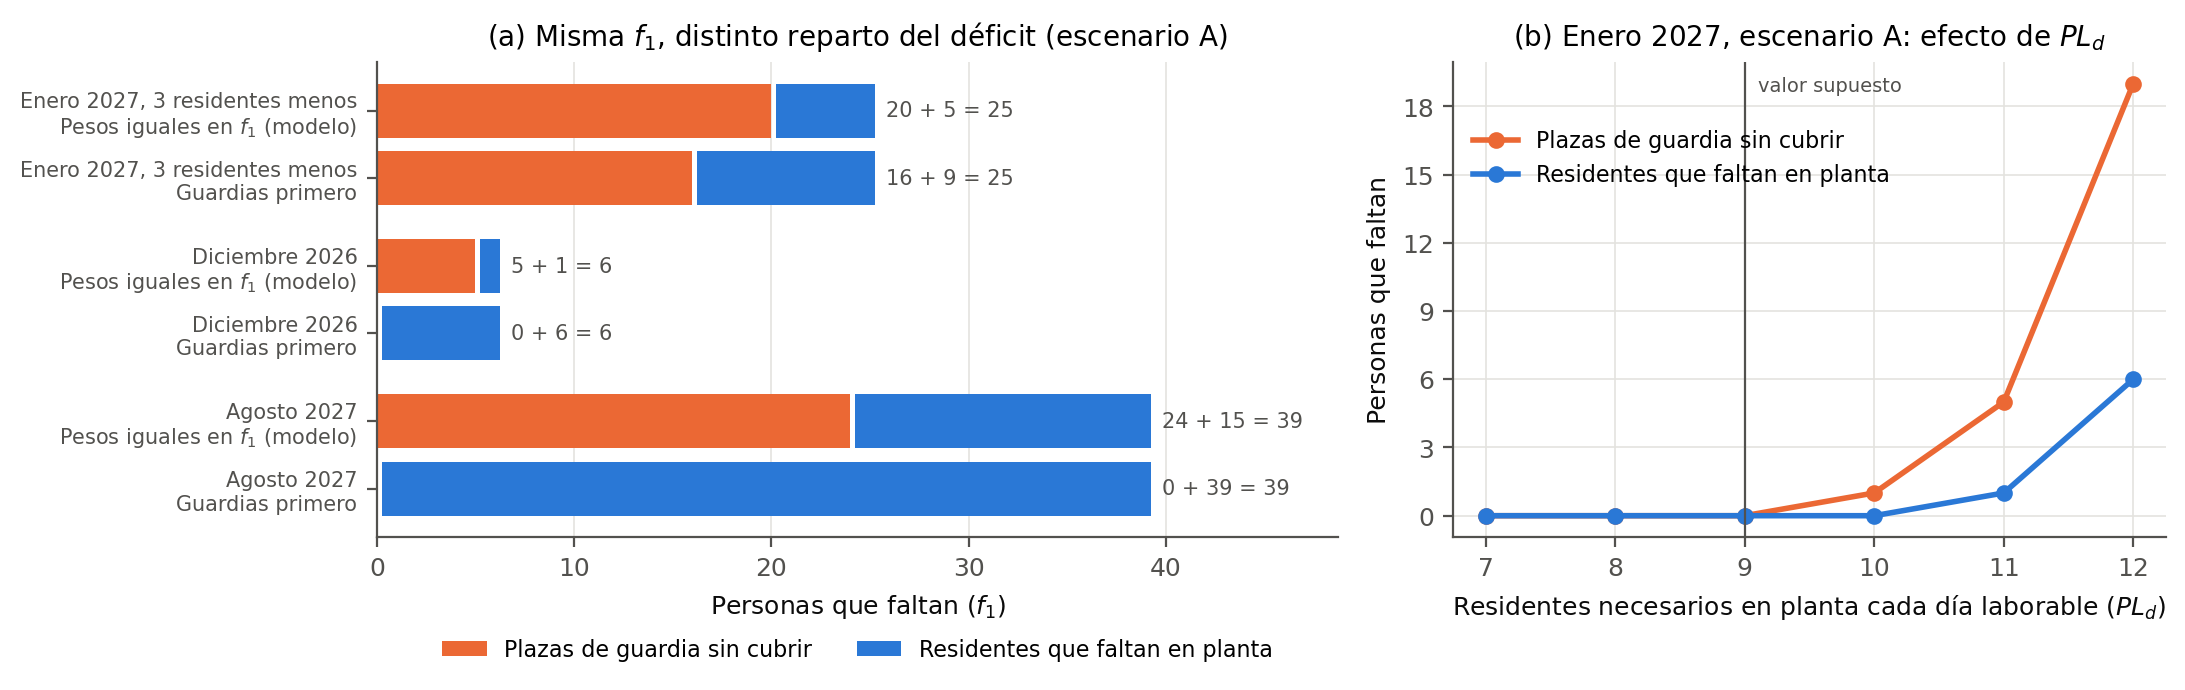
\includegraphics[width=\linewidth]{final_duties_vs_ordinary.png}
\caption{(a) Reparto del déficit $f_1$ entre guardias sin cubrir y residentes que faltan en planta, con el modelo (pesos iguales) y cubriendo primero las guardias. (b) Efecto del número de residentes necesarios en planta cada día laborable ($PL_d$) en enero de 2027, escenario A.}
\label{fig:planta}
\end{figure}

\begin{itemize}
  \item \textbf{El déficit total no cambia, cambia dónde cae} (Figura~\ref{fig:planta}a). En diciembre pasamos de 5 guardias sin cubrir y 1 residente menos en planta a 0 guardias sin cubrir y 6 residentes menos en planta; en agosto, de $24 + 15$ a $0 + 39$. Cada guardia cubierta cuesta un residente-día en planta: el intercambio es 1 a 1.
  \item \textbf{Con la plantilla actual, agosto se puede cubrir} si el servicio acepta tener de media 1,8 residentes menos en planta cada día laborable (39 residentes-día en 22 días laborables). El precio es también el cansancio: cubrir todas las guardias obliga a 16 patrones «día sí, día no» frente a ninguno.
  \item \textbf{Cuando el límite es la capacidad de guardias}, priorizar las guardias ayuda poco: con 3 residentes menos en enero las plazas sin cubrir solo bajan de 20 a 16, que es $93 - 11 \times 7$, el mínimo posible.
  \item \textbf{El requisito de planta supuesto ($PL_d = 9$) está justo en el límite} (Figura~\ref{fig:planta}b). Con $PL_d \le 9$ guardias y planta no compiten en enero; con 10 queda 1 guardia sin cubrir, con 11 quedan 5 guardias y 1 residente en planta, y con 12 el déficit sube a 25. Es uno de los parámetros que más conviene validar con el servicio.
\end{itemize}

\textbf{Implicación.} Que una guardia sin cubrir y un residente menos en planta pesen igual no es una verdad técnica sino una decisión de gestión. Si la urgencia no puede quedar descubierta, el servicio debe usar la variante «guardias primero» y planificar en verano una actividad ordinaria reducida; el modelo dice exactamente cuánta.

\subsection{Equidad a lo largo de varios meses}
\label{sec:equidad}

En un solo mes la equidad mejora poco (Sección~\ref{sec:resultados}). Para ver el efecto a medio plazo, simulamos cinco meses seguidos (enero a mayo de 2027): tras cada mes, el histórico $H_r$, la disponibilidad $\Phi_r$ y las guardias de los dos últimos días ($Y_{rd}$) se actualizan con el cuadrante que acaba de producir el modelo. Comparamos cuatro políticas, evaluadas siempre con la carga acumulada real de cada residente:
\begin{enumerate}
  \item \textbf{Rango con memoria} (el modelo de la Sección~\ref{sec:modelo}).
  \item \textbf{Desviación media con memoria}: $f_3$ se sustituye por la desviación absoluta media de las cargas normalizadas respecto a su media, una métrica alternativa que tiene en cuenta a todos los residentes y no solo a los extremos.
  \item \textbf{Rango sin memoria}: cada mes se equilibra por separado ($H_r = 0$), como haría quien reparte bien los festivos de cada mes sin mirar los anteriores.
  \item \textbf{Sin criterio de equidad}: $f_3$ eliminado.
\end{enumerate}

\begin{figure}[ht]
\centering
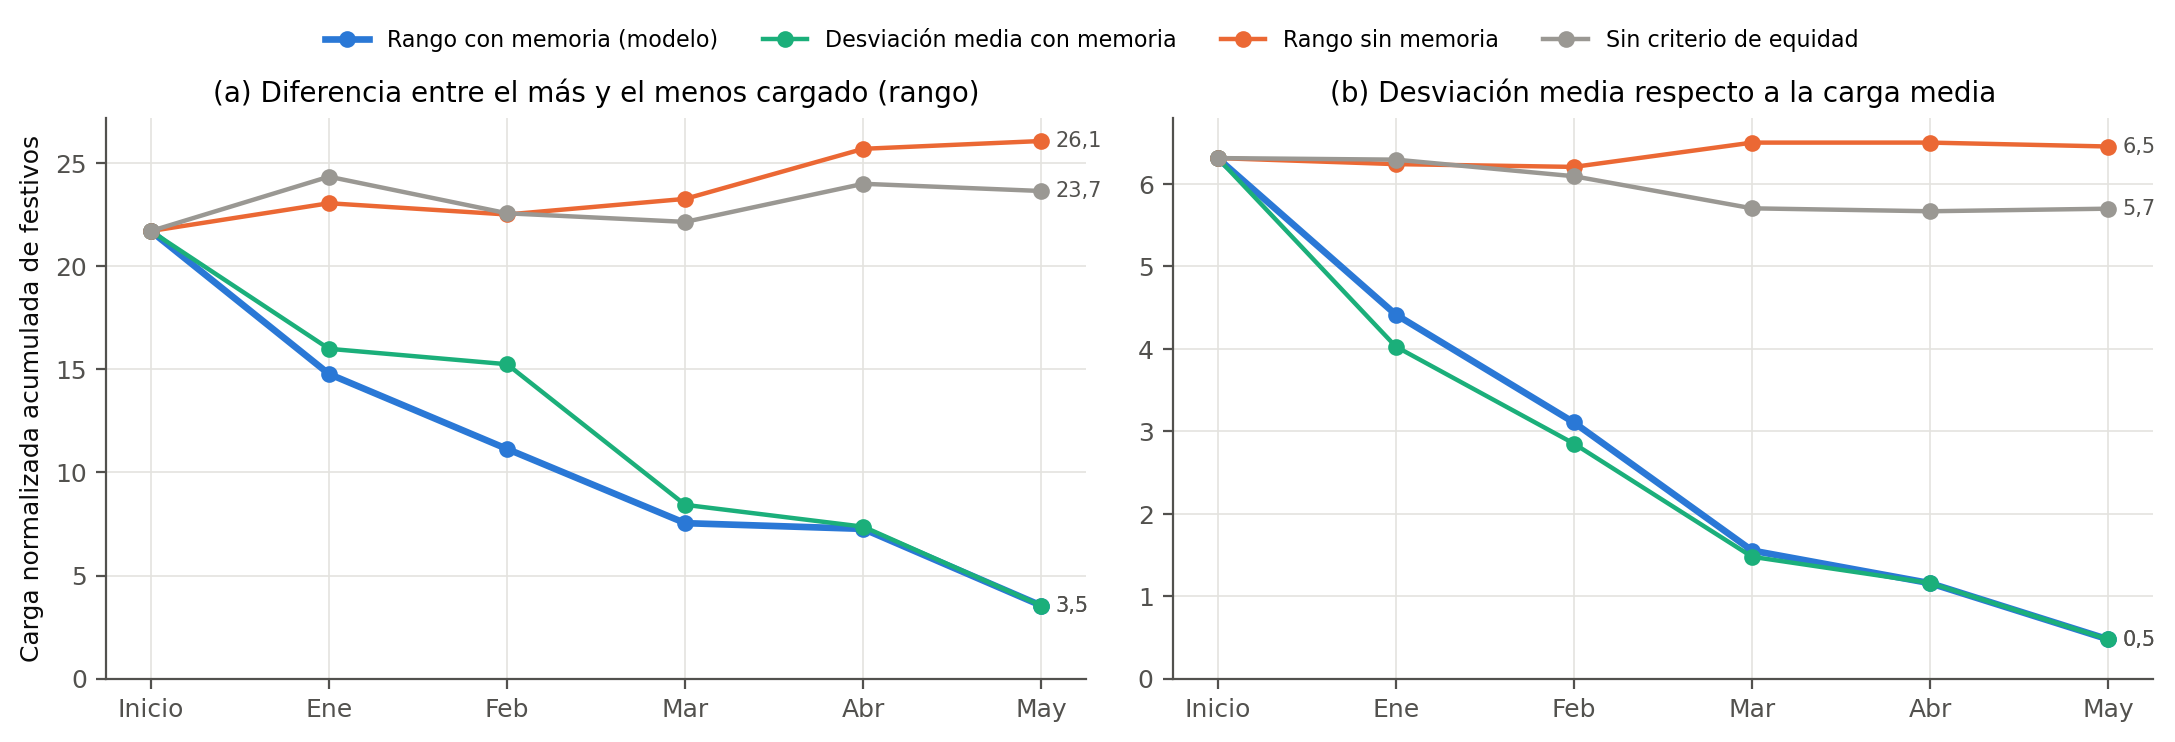
\includegraphics[width=\linewidth]{final_fairness_rolling.png}
\caption{Desigualdad en la carga acumulada de guardias en fin de semana o festivo (normalizada por disponibilidad) a lo largo de cinco meses: (a) diferencia entre el residente más cargado y el menos cargado; (b) desviación absoluta media respecto a la carga media.}
\label{fig:rolling}
\end{figure}

% Numbers from results/tables/final_fairness_rolling.csv (notebook 03, Section 3.4).
\begin{itemize}
  \item \textbf{Con memoria, la desigualdad se reduce mes a mes} (Figura~\ref{fig:rolling}). Con el modelo, la diferencia entre el más y el menos cargado pasa de 21,7 al principio a 14,8 tras enero y a 3,5 tras mayo, y la desviación media baja de 6,3 a 0,5. No cuesta nada: en los cinco meses se cubren todas las guardias ($f_1 = 0$) y se respetan todas las peticiones ($f_2 = 0$).
  \item \textbf{Sin memoria no se corrige nada.} Equilibrar cada mes por separado deja la desigualdad acumulada igual o peor que no tener ningún criterio de equidad: tras mayo el rango es 26,1 sin memoria y 23,7 sin criterio, frente a 3,5 con memoria. Repartir bien los festivos de cada mes da los mismos festivos a quien ya arrastraba un exceso que a quien iba por detrás: \emph{la memoria es lo que hace justo el reparto}.
  \item \textbf{La métrica importa poco a medio plazo.} La desviación media reparte mejor entre los residentes intermedios al principio (4,0 frente a 4,4 tras enero) y el rango protege mejor al más cargado (14,8 frente a 16,0), pero tras cinco meses ambas llegan al mismo reparto (rango 3,5). Recomendamos mantener el rango: es más fácil de explicar («la diferencia entre quien más y quien menos festivos lleva») y se resuelve en menos de un segundo, mientras que la desviación media tarda hasta 36~s en algunos meses.
  \item \textbf{El rango de un solo mes engaña.} En enero el rango se queda en 14,8 aunque cambie la plantilla (Sección~\ref{sec:plantilla}), porque lo fija el residente con más histórico. Visto a lo largo de varios meses el criterio sí funciona: lo que no se puede compensar en un mes se compensa en los siguientes.
\end{itemize}

{\small Detalle técnico: para esta simulación los niveles del objetivo se resuelven uno a uno, con 20~s cada uno. La política sin memoria agota ese límite en el nivel de equidad (tiene muchas soluciones simétricas); las demás se resuelven hasta optimalidad probada.\par}


\subsection{¿Qué aporta cada objetivo?}
\label{sec:objetivos}

Quitamos cada objetivo de menor prioridad por turnos y comparamos el orden lexicográfico con la suma ponderada $1000 f_1 + 100 f_2 + 10 f_3 + f_4$ (Tabla~\ref{tab:objetivos}).

\begin{table}[ht]
\centering\small
\caption{Qué aporta cada objetivo (escenario A). Cada fila elimina un objetivo de menor prioridad o sustituye el orden lexicográfico por la suma ponderada $1000 f_1 + 100 f_2 + 10 f_3 + f_4$.}
\label{tab:objetivos}
\begin{tabular}{@{}llccccc@{}}
\toprule
Mes & Variante & \makecell{$f_1$ (guardias sin\\ cubrir + planta)} & \makecell{Peticiones\\ incumplidas} & \makecell{Rango de\\ festivos $f_3$} & \makecell{Patrones\\ $f_4$} & \makecell{Tiempo\\ (s)} \\
\midrule
\multirow{5}{*}{Enero 2027} & Modelo (lexicográfico) & 0 (0 + 0) & 0/17 & 14{,}8 & 1 & 0{,}3 \\
 & Sin $f_2$ (peticiones) & 0 (0 + 0) & 4/17 & 14{,}8 & 1 & 0{,}3 \\
 & Sin $f_3$ (equidad) & 0 (0 + 0) & 0/17 & 24{,}4 & 0 & 0{,}2 \\
 & Sin $f_4$ (día sí, día no) & 0 (0 + 0) & 0/17 & 14{,}8 & 16 & 0{,}2 \\
 & Suma ponderada & 0 (0 + 0) & 0/17 & 14{,}9 & 0 & 0{,}2 \\
\midrule
\multirow{5}{*}{Diciembre 2026} & Modelo (lexicográfico) & 6 (5 + 1) & 0/12 & 23{,}1 & 0 & 0{,}3 \\
 & Sin $f_2$ (peticiones) & 6 (5 + 1) & 4/12 & 23{,}1 & 0 & 0{,}2 \\
 & Sin $f_3$ (equidad) & 6 (6 + 0) & 0/12 & 29{,}0 & 0 & 0{,}2 \\
 & Sin $f_4$ (día sí, día no) & 6 (6 + 0) & 0/12 & 23{,}1 & 23 & 0{,}2 \\
 & Suma ponderada & 6 (5 + 1) & 0/12 & 23{,}1 & 0 & 0{,}1 \\
\midrule
\multirow{5}{*}{Agosto 2027} & Modelo (lexicográfico) & 39 (24 + 15) & 0/21 & 9{,}8 & 0 & 0{,}2 \\
 & Sin $f_2$ (peticiones) & 39 (21 + 18) & 4/21 & 5{,}5 & 1 & 0{,}2 \\
 & Sin $f_3$ (equidad) & 39 (24 + 15) & 0/21 & 13{,}2 & 0 & 0{,}2 \\
 & Sin $f_4$ (día sí, día no) & 39 (22 + 17) & 0/21 & 9{,}8 & 14 & 0{,}2 \\
 & Suma ponderada & 39 (21 + 18) & 0/21 & 9{,}8 & 0 & 0{,}1 \\
\bottomrule
\end{tabular}
\end{table}


\begin{itemize}
  \item \textbf{Las peticiones y los patrones salen gratis en cobertura.} Sin $f_2$ el modelo incumple 4 peticiones en cada mes sin reducir en nada los requisitos incumplidos $f_1$; sin $f_4$ aparecen 16, 23 y 14 patrones «día sí, día no» donde el modelo deja 1, 0 y 0. Los dos objetivos cambian mucho la calidad del cuadrante para los residentes sin coste para el servicio.
  \item \textbf{En agosto, peticiones y equidad compiten.} Si se ignoran las peticiones, el rango de festivos baja de 9,8 a 5,5 a cambio de incumplir 4 de 21 peticiones. El orden de prioridades (peticiones antes que equidad) es una decisión que el servicio debe tomar conscientemente; el modelo cuantifica su precio.
  \item \textbf{Sin criterio de equidad} el rango acumulado de festivos empeora incluso respecto al de partida en enero (de 21,7 a 24,4) y en diciembre (de 27,5 a 29,0).
  \item \textbf{La suma ponderada no respeta las prioridades.} En enero cambia equidad por patrones (rango 14,9 en lugar de 14,8, a cambio de quitar un patrón, porque $10 \times 0{,}08 < 1$). En agosto alcanza el mismo $f_1 = 39$ pero lo reparte de otra forma ($21 + 18$ en lugar de $24 + 15$): entre soluciones empatadas elige de forma arbitraria. El orden lexicográfico evita tener que calibrar pesos y se resuelve igual de rápido.
\end{itemize}

\subsection{Validez y limitaciones del análisis}

\begin{itemize}
  \item \textbf{Datos sintéticos.} Las cifras dependen de los supuestos de la Tabla~\ref{tab:supuestos}. Los mecanismos (el coste de los salientes, el límite aritmético en B, el efecto de la memoria) son robustos; las cifras exactas deben recalcularse con los datos del servicio. Los parámetros más influyentes son $PL_d$, los límites mensuales y la estructura de guardias.
  \item \textbf{Escenario B aproximado.} Suponer que todas las guardias son de 17~h ignora que las de 24~h de fin de semana tendrán que partirse en dos módulos, lo que probablemente aumentará las necesidades. Tampoco modelamos el descanso semanal de 24~h ni la media de 45~h semanales del RD 951/2026, porque no modelamos el horario de la jornada ordinaria.
  \item \textbf{Residentes añadidos optimistas.} Los residentes sintéticos añadidos están disponibles todo el mes; uno real también tendría vacaciones, así que las cifras de la Tabla~\ref{tab:plantilla} para agosto son una cota inferior.
  \item \textbf{Varios cuadrantes óptimos.} Los valores de $f_1$ a $f_4$ son únicos, pero puede haber varios cuadrantes que los alcancen. Indicadores que no se optimizan (como el reparto de guardias por residente) pueden cambiar entre ejecuciones o versiones del solver; si el servicio los considera importantes, deberían convertirse en objetivos.
\end{itemize}

% =====================================================================
\section{Conclusiones y recomendaciones}
\label{sec:conclusiones}

Hemos formulado el cuadrante mensual de guardias de residentes como un modelo de programación entera con cuatro objetivos jerarquizados que \emph{siempre} devuelve un cuadrante: si el mes no se puede cubrir, dice exactamente qué falta y cuándo. El modelo se resuelve en menos de un segundo y cada cuadrante se valida de forma independiente. Respondiendo a las preguntas del inicio:

\begin{enumerate}[label=\textbf{P\arabic*.}]
  \item \textbf{Cobertura.} En un mes normal la plantilla actual lo cubre todo, respeta todas las peticiones y casi no genera patrones agotadores, pero sin ningún margen. En diciembre y agosto quedan huecos (6 y 39 requisitos) que el modelo localiza día a día.
  \item \textbf{Plantilla.} Con el RD 951/2026 y la estructura de guardias actual el servicio necesita unos 24 residentes disponibles en lugar de 14. En el régimen actual necesita 16 en Navidad y 19 en agosto para cumplir también con la actividad ordinaria, o puede cubrir todas las guardias con los 14 actuales reduciendo la actividad ordinaria.
  \item \textbf{Equidad.} Equilibrar cada mes por separado no corrige un reparto heredado injusto; con memoria, la desigualdad acumulada se reduce mes a mes.
  \item \textbf{Prioridades.} Respetar las peticiones y evitar los patrones «día sí, día no» no cuesta cobertura. Las decisiones con un precio real son dos: guardias frente a actividad ordinaria y, en meses tensos, peticiones frente a equidad.
\end{enumerate}

\paragraph{Recomendaciones para el servicio.}
\begin{enumerate}
  \item \textbf{Usar el modelo cada mes} en lugar del cuadrante manual: da un cuadrante óptimo y auditable en segundos y señala los huecos con antelación.
  \item \textbf{Preparar ya la transición a septiembre de 2027.} Con la estructura actual harían falta unos 10 residentes más. El servicio debería decidir entre ampliar la plantilla y rediseñar las guardias (menos plazas cubiertas por residentes, módulos más cortos o más adjuntos) y usar el modelo para comparar las propuestas.
  \item \textbf{Decidir explícitamente qué va primero en verano}: la urgencia o la actividad ordinaria. Si es la urgencia, programar en agosto una actividad ordinaria reducida (unos 2 residentes menos al día) y escalonar las vacaciones para que no coincidan.
  \item \textbf{Mantener la equidad con memoria a lo largo del año de residencia}, que es lo que corrige los desequilibrios heredados.
  \item \textbf{Validar con el servicio los parámetros más influyentes}: residentes necesarios en planta, límites mensuales, quién cuenta como mayor y la nueva estructura de guardias.
\end{enumerate}

\paragraph{Trabajo futuro.} (i) Validar los supuestos y recalcular los resultados con datos reales del hospital. (ii) Modelar el escenario B con los nuevos tipos de guardia y su duración $T_g$ (restricción 10 completa). (iii) Reprogramar ante ausencias imprevistas con el mínimo número de cambios, $\min \sum |x_{rdg} - \hat x_{rdg}|$, y evaluar la robustez del cuadrante con simulación Monte Carlo de bajas.
